\documentclass[numbers=enddot,12pt,final,onecolumn,notitlepage]{scrartcl}%
\usepackage[paperwidth=21cm,paperheight=195cm,margin=1in]{geometry}
\usepackage{amsmath}
\usepackage{amssymb}
\usepackage{array}
\usepackage{setspace}
\usepackage{graphicx}
\usepackage{etex}
\usepackage{amsthm}
\usepackage{color}
\usepackage{wasysym}
\usepackage[all]{xy}
\usepackage{textpos}
%\usepackage{ytableau}
\usepackage{stmaryrd}
\usepackage{url}
\usepackage{color}
\usepackage{epsfig,amsfonts,mathrsfs}
\usepackage{verbatim}
\usepackage{xparse}
\usepackage{amsfonts}
\usepackage{tcolorbox}
\usepackage{hyperref}%
\setcounter{MaxMatrixCols}{30}
%TCIDATA{OutputFilter=latex2.dll}
%TCIDATA{Version=5.50.0.2960}
%TCIDATA{LastRevised=Wednesday, July 08, 2020 00:42:26}
%TCIDATA{<META NAME="GraphicsSave" CONTENT="32">}
%TCIDATA{<META NAME="SaveForMode" CONTENT="1">}
%TCIDATA{BibliographyScheme=Manual}
%BeginMSIPreambleData
\providecommand{\U}[1]{\protect\rule{.1in}{.1in}}
%EndMSIPreambleData
\definecolor{grau}{rgb}{.5 , .5 , .5}
\definecolor{dunkelgrau}{rgb}{.35 , .35 , .35}
\definecolor{schwarz}{rgb}{0 , 0 , 0}
\definecolor{violet}{RGB}{143,0,255}
\definecolor{forestgreen}{RGB}{34, 100, 34}

\newcommand{\ssty}{\scriptstyle}
\newcommand{\w}{\omega}
\newcommand{\sr}{\stackrel}
\newcommand{\ov}{\overline}
\newcommand{\ga}{\gamma}
\newcommand{\al}{\alpha}
\newcommand{\be}{\beta}
\newcommand{\si}{\sigma}
\newcommand{\la}{\lambda}
\newcommand{\eps}{\varepsilon}
\newcommand{\CC}{\mathbb{C}} % complex numbers
\newcommand{\RR}{\mathbb{R}} % real numbers
\newcommand{\QQ}{\mathbb{Q}} % rational numbers
\newcommand{\NN}{\mathbb{N}} % nonnegative integers
\newcommand{\PP}{\mathbb{P}} % positive integers
\newcommand{\ZZ}{\mathbb{Z}} % integers
\newcommand{\id}{\operatorname{id}} % identity map
\newcommand{\kk}{\mathbf{k}} % our base ring
\newcommand{\QSym}{\operatorname{QSym}}
\newcommand{\Des}{\operatorname{Des}}
\newcommand{\Odd}{\operatorname{Odd}}
\newcommand{\Comp}{\operatorname{Comp}}
\newcommand{\Peak}{\operatorname{Peak}}

% For shuffle product symbol
\makeatletter
\providecommand*{\shuffle}{%
  \mathbin{\mathpalette\shuffle@{}}%
}
\newcommand*{\shuffle@}[2]{%
  % #1: math style
  % #2: unused
  \sbox0{$#1\vcenter{}$}%
  \kern .15\ht0 % side bearing
  \rlap{\vrule height .25\ht0 depth 0pt width 2.5\ht0}%
  \raise.1\ht0\hbox to 2.5\ht0{%
    \vrule height 1.75\ht0 depth -.1\ht0 width .17\ht0 %
    \hfill
    \vrule height 1.75\ht0 depth -.1\ht0 width .17\ht0 %
    \hfill
    \vrule height 1.75\ht0 depth -.1\ht0 width .17\ht0 %
  }%
  \kern .15\ht0 % side bearing
}

\makeatother


\newcommand{\red}{\color{red}}
\newcommand{\grey}{\color{grau}}
\newcommand{\green}{\color{forestgreen}}
\newcommand{\violet}{\color{violet}}
\newcommand{\blue}{\color{blue}}
\newcommand{\EE}{{\mathbf{E}}}
\newcommand{\OO}{\operatorname {O}}
\newcommand{\Nm}{\operatorname {N}}
\newcommand{\Par}{\operatorname{Par}}
\newcommand{\Stab}{\operatorname {Stab}}
\newcommand{\ev}{\operatorname{ev}}
\newcommand{\Sym}{\operatorname{Sym}}
\newcommand{\des}{\operatorname{des}}
\newcommand{\inv}{\operatorname{inv}}
\newcommand{\maj}{\operatorname{maj}}
\newcommand{\NSym}{\operatorname{NSym}}
\newcommand{\Gr}{\operatorname{Gr}}
\newcommand{\QHo}{\operatorname{QH}}
\newcommand{\Ho}{\operatorname{H}}
\newcommand{\Mat}{\operatorname{M}}
\newcommand{\bk}{\mathbf{k}}
\newcommand{\Nplus}{\mathbb{N}_{+}}
\newcommand\arxiv[1]{\href{http://www.arxiv.org/abs/#1}{\texttt{arXiv:#1}}}
\newcommand{\GL}{\operatorname {GL}}
\newcommand{\SL}{\operatorname {SL}}
\newcommand{\Or}{\operatorname {O}}
\newcommand{\im}{\operatorname {Im}}
\newcommand{\Iso}{\operatorname {Iso}}
\newcommand{\Adm}{\operatorname{Adm}}
\newcommand{\Supp}{\operatorname{Supp}}
\newcommand{\Powser}{\QQ\left[\left[x_1,x_2,x_3,\ldots\right]\right]}
\newcommand{\rad}{\operatorname {rad}}
\newcommand{\zero}{\mathbf{0}}
\newcommand{\xx}{\mathbf{x}}
\newcommand{\ord}{\operatorname*{ord}}
\newcommand{\bbK}{{\mathbb{K}}}
\newcommand{\whP}{{\widehat{P}}}
\newcommand{\calP}{\mathcal{P}}
\newcommand{\calS}{\mathcal{S}}
\newcommand{\calZ}{\mathcal{Z}}
\newcommand{\calA}{\mathcal{A}}
\newcommand{\calL}{\mathcal{L}}
\newcommand{\lcm}{\operatorname*{lcm}}
\newcommand{\lm}{\lambda / \mu}
\newcommand{\fti}[1]{\subsection{#1}}
\newenvironment{iframe}[1][]{ \fti{[#1]} \begin{itemize}}{\end{itemize}}
\newcommand{\are}{\ar@{-}}
\newcommand{\arinj}{\ar@{_{(}->}}
\newcommand{\arsurj}{\ar@{->>}}
\newcommand{\set}[1]{\left\{ #1 \right\}}
\newcommand{\abs}[1]{\left| #1 \right|}
\newcommand{\tup}[1]{\left( #1 \right)}
\newcommand{\ive}[1]{\left[ #1 \right]}
\newcommand{\verts}[1]{\operatorname{V}\left( #1 \right)}
\newcommand{\edges}[1]{\operatorname{E}\left( #1 \right)}
\newcommand{\arcs}[1]{\operatorname{A}\left( #1 \right)}
\newcommand{\underbrack}[2]{\underbrace{#1}_{\substack{#2}}}
\definecolor{darkred}{rgb}{0.7,0,0}
\newcommand{\defn}[1]{{\color{darkred}\emph{#1}}}
\newcommand{\defnm}[1]{{\color{darkred} #1}}
\newcommand{\STRUT}{\vrule width 0pt depth 8pt height 0pt}
\newcommand{\ASTRUT}{\vrule width 0pt depth 0pt height 11pt}
\newcommand{\iso}{\cong}
\newcommand{\fs}{\mathcal{S}}
\newcommand{\mbf}{\mathbf}
\newcommand{\0}{\phantom{c}}
\newcommand{\swt}[1]{\left\langle #1 \right\rangle}
\newcommand{\SymGp}[1]{\mathfrak{S}_{#1}}
\DeclareMathOperator{\wt}{wt}
\newcommand{\wtg}{\widetilde{g}}
\newcommand{\cont}{\operatorname{cont}}
\newcommand{\ircont}{\operatorname{ircont}}
\newcommand{\ceq}{\operatorname{ceq}}
\newcommand{\ttt}{{\mathbf{t}}}
\newcommand{\mm}{\mathbf{m}}
\newcommand{\nn}{\mathbf{n}}
\newcommand{\qq}{\mathbf{q}}
\newcommand{\mcA}{\mathcal{A}}
\newcommand{\mcF}{\mathcal{F}}
\newcommand{\mcM}{\mathcal{M}}
\newcommand{\mcW}{\mathcal{W}}
\newcommand{\mcI}{\mathcal{I}}
\let\sumnonlimits\sum
\let\prodnonlimits\prod
\let\cupnonlimits\bigcup
\let\capnonlimits\bigcap
\renewcommand{\sum}{\sumnonlimits\limits}
\renewcommand{\prod}{\prodnonlimits\limits}
\renewcommand{\bigcup}{\cupnonlimits\limits}
\renewcommand{\bigcap}{\capnonlimits\limits}
\renewcommand{\labelitemii}{$\spadesuit$}
\newcommand{\nowbox}{\hphantom{x} \vspace{-1.5pc}}

\tcbuselibrary{theorems}
\newtcbtheorem
  []% init options
  {definition}% name
  {Definition}% title
  {%
    colback=green!5,
    colframe=green!35!black,
    fonttitle=\bfseries,
  }% options
  {def}% prefix

\newtcbtheorem
  []% init options
  {theorem}% name
  {Theorem}% title
  {%
    colback=cyan!5,
    colframe=cyan!75!black,
    fonttitle=\bfseries,
  }% options
  {def}% prefix

\newtcbtheorem
  []% init options
  {corollary}% name
  {Corollary}% title
  {%
    colback=blue!5,
    colframe=blue!35!black,
    fonttitle=\bfseries,
  }% options
  {def}% prefix

\newtcbtheorem
  []% init options
  {proposition}% name
  {Proposition}% title
  {%
    colback=blue!5,
    colframe=blue!35!black,
    fonttitle=\bfseries,
  }% options
  {def}% prefix

\newtcbtheorem
  []% init options
  {question}% name
  {Question}% title
  {%
    colback=red!5,
    colframe=red!35!black,
    fonttitle=\bfseries,
  }% options
  {def}% prefix

\newtcbtheorem
  []% init options
  {problem}% name
  {Problem}% title
  {%
    colback=red!5,
    colframe=red!35!black,
    fonttitle=\bfseries,
  }% options
  {def}% prefix

\newtcbtheorem
  []% init options
  {conjecture}% name
  {Conjecture}% title
  {%
    colback=red!5,
    colframe=red!35!black,
    fonttitle=\bfseries,
  }% options
  {def}% prefix

\iffalse
\NOEXPAND{\defn}[1]{\defn}
\NOEXPAND{\defnm}[1]{\defnm}
\fi

\usepackage[backend=bibtex]{biblatex}
\addbibresource{biblio.bib}

\begin{document}

\title{Weighted posets and the enriched monomial basis of QSym [slides]}
\author{\href{http://www.cip.ifi.lmu.de/~grinberg/}{Darij Grinberg} and Ekaterina Vassilieva}
\date{2022-01-17}
\maketitle

\noindent \textbf{these slides: \color{red}
\url{https://github.com/darijgr/fpsac21eta/raw/main/fps21eta-talk.pdf}}%
\newline\textbf{paper: \color{red}
\url{https://www.mat.univie.ac.at/~slc/wpapers/FPSAC2021/58Grinberg.pdf}}%
\newline

\begin{tcolorbox}[colback=cyan!5,colframe=cyan!75!black, fonttitle=\bfseries,title=Summary of our work] Hsiao defines in \cite{Hsi07} the \textbf{monomial peak functions} $\eta_{\al}$: a class of quasisymmetric functions indexed by \textbf{odd compositions} of $n$.
\begin{equation*}
\eta_{\al} = (-1)^{(n-\ell(\al))/2}\sum\limits_{\substack{i_1 \leq \dots \leq i_p}}2^{|\{i_1,i_2,\dots,i_p\}|} x_{i_1}^{\al_1}x_{i_2}^{\al_2} \cdots x_{i_p}^{\al_p}.
\end{equation*}
They provide a monomial-like basis to Stembridge's algebra of peaks \cite{Ste97} and are related to Stembridge peak functions $K_\al$ through
\begin{equation*}
K_{\al} = \sum_{{\substack{\beta \in \Odd(n);\\ \Peak(\beta) \subseteq \Peak(\al)}}} \eta_{\beta}.
\end{equation*}
In the present work: 
\begin{itemize}
\item We show that monomial peak functions may be extended to \textbf{a basis of (the whole) QSym}. We name this new basis the \textbf{enriched monomial basis} of QSym.
\item We relate it to other bases of QSym, compute its \textbf{antipode} and \textbf{coproduct}. 
\item We introduce \textbf{weighted posets} and their \textbf{enriched P-partitions} (generalizing both the weighted posets of 
\cite{Gri17} and the enriched P-partitions of \cite{Ste97}), whose generating functions give a \textbf{universal framework} for many types of quasisymmetric functions.

\begin{center}
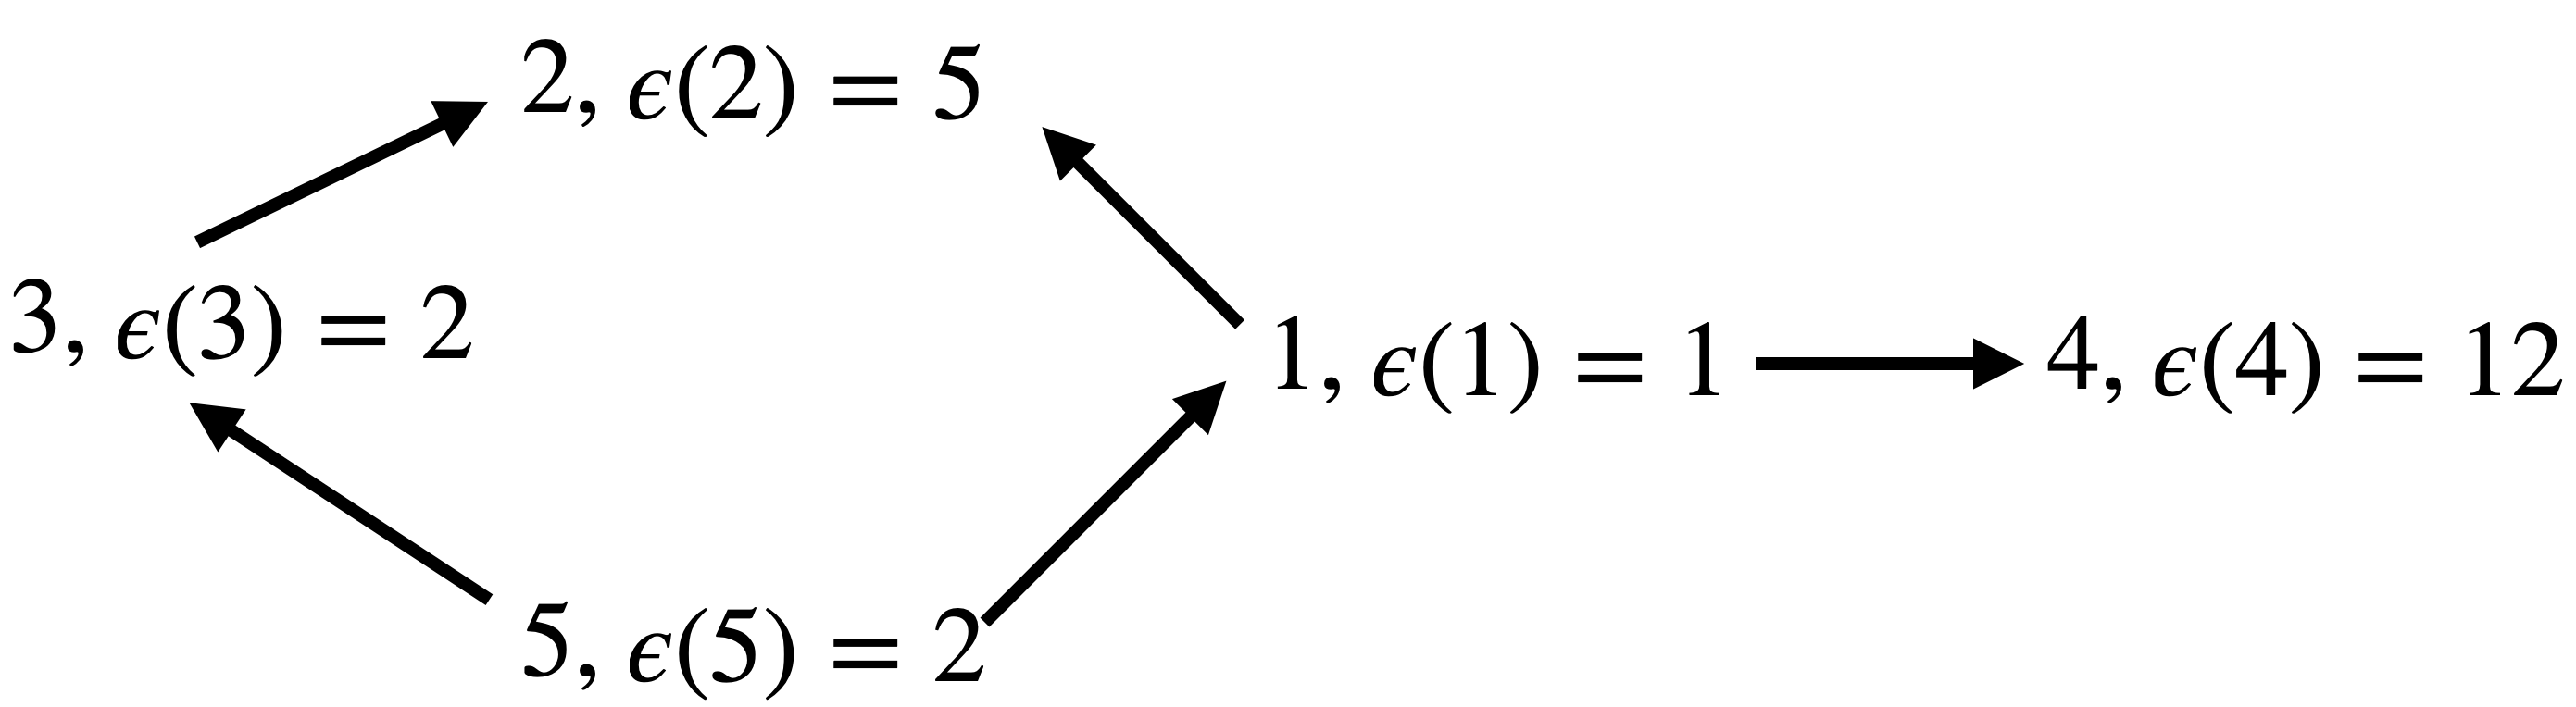
\includegraphics[scale=0.16]{Poset.png}
\end{center}
 
\item We use our framework to compute the \textbf{product} of two enriched monomials:
\begin{equation*}
\eta_\al \eta_\beta
= \sum_{\substack{\gamma \in \al \shuffle \be ;\\
                   I\subseteq \left(S_{\be}(\gamma)\setminus (S_{\be}(\gamma)-1)\right) \setminus \left\{1\right\}}}
(-1)^{|I|}\eta_{\gamma^{\downarrow\downarrow I}} .
\end{equation*}
\end{itemize}
\end{tcolorbox}

%%%%%%%%%%%%%%%%%%%%%%%%%%%%%%%%%%
%%%%%%%%%%%%%%%%%%%%%%%%%%%%%%%%%%
%%%%%%%%%%%%%%%%%%%%%%%%%%%%%%%%%%
\section{Notation and basic definitions}
%%%%%%%%%%%%%%%%%%%%%%%%%%%%%%%%%%
%%%%%%%%%%%%%%%%%%%%%%%%%%%%%%%%%%
%%%%%%%%%%%%%%%%%%%%%%%%%%%%%%%%%%


%%%%%%%%%%%%%%%%%%%%%%%%%%%%%%%%%%
\subsection{Compositions and permutations statistics}
%%%%%%%%%%%%%%%%%%%%%%%%%%%%%%%%%%

\begin{itemize}
\item $\defnm{\PP} =\left\{1,2,\dots\right\}$, $\defnm{\NN} = \left\{0,1,\ldots\right\}$, $\defnm{[n]} = \left\{1,2,\dots, n\right\}$, $\defnm{S_n}$ the symmetric group on $[n]$.

\item \defn{$\Comp(n)$} is the set of \defn{compositions} $\al = (\al_1, \al_2, \dots, \al_p)$ of $n$. \defn{$\Odd(n)$} is the set of \defn{odd compositions} of $n$ containing only odd integers.  Let $\ell(\al) := p$, $|\al| := \sum_i \al_i = n$.

\item The \defn{descent set} $\Des(\pi)$ of $\pi \in S_n$ is 
$\Des(\pi) = \{1\leq i\leq n-1| \pi(i)>\pi(i+1)\}.$


\item The \defn{peak set} $\Peak(\pi)$ of $\pi$ is $
\Peak(\pi) = \{2\leq i\leq n-1| \pi(i-1)<\pi(i)>\pi(i+1)\}.$

\item Compositions of $n$ are in bijection with descent sets of permutations in $S_n$, while odd compositions of $n$ are in (a more complicated) bijection with peak sets. Denote \defn{$\Des(\al)$} (resp. \defn{$\Peak(\al)$}) the descent set (resp., peak set) associated with composition (resp., odd composition) $\al$.

\end{itemize}

%%%%%%%%%%%%%%%%%%%%%%%%%%%%%%%%%%
\subsection{Quasisymmetric functions}
%%%%%%%%%%%%%%%%%%%%%%%%%%%%%%%%%%


\begin{itemize}
\item For any $n \in \NN$ and $\al =(\al_1,\al_2,\dots,\al_p) \in \Comp(n)$, define the \defn{monomial quasisymmetric function} $M_\al$ and the \defn{fundamental quasisymmetric function} $L_\al$ by

\begin{equation*}
\label{eq : M+L}
M_{\al} = \sum\limits_{i_1 < \cdots < i_p} x_{i_1}^{\al_1}x_{i_2}^{\al_2} \cdots x_{i_p}^{\al_p},\;\;\;\;\;\;\qquad L_{\al} = \sum\limits_{\substack{i_1 \leq \cdots \leq i_n;\\j\in \Des(\al) \implies i_j<i_{j+1}}} x_{i_1}x_{i_2} \cdots x_{i_n}.
\end{equation*}

\item As an example, for $n=3$, we have
\begin{gather*}
M_{(2,1)}=\sum_{i<j}x_{i}^{2}x_{j}=x_{1}^{2}x_{2}+x_{1}%
^{2}x_{3}+x_{2}^{2}x_{3}+x_{1}^{2}x_{4}+x_{2}^{2}x_{4}+x_{3}^{2}x_{4}+\dots,\\
L_{(2,1)}=\sum_{i\leq j <k}x_{i}x_{j}x_k=x_{1}^{2}x_{2}+x_{1}%
^{2}x_{3}+x_{1}x_{2}x_3+x_{2}^{2}x_{3}+x_{1}^{2}x_{4}+x_{1}
x_{2}x_{4}+x_{2}^{2}x_{4}+\dots.
\end{gather*}
\item The sets $\left\{M_\al\right\}_{n\in \NN,\ \al\in \Comp(n)}$
and $\left\{L_\al\right\}_{n\in \NN,\ \al\in \Comp(n)}$
are two bases of the $\kk$-module $\QSym$ of quasisymmetric functions.
They are related through
\begin{equation}
\label{eq : LM} L_{\al} = \sum_{{\substack{\beta \in \Comp(n);\\\Des(\alpha) \subseteq \Des(\beta)}}} M_{\beta}.
\end{equation}
\end{itemize}

%%%%%%%%%%%%%%%%%%%%%%%%%%%%%%%%%%
\subsection{Peak and monomial peak functions}
%%%%%%%%%%%%%%%%%%%%%%%%%%%%%%%%%%

\begin{itemize}
\item In \cite{Ste97}, Stembridge introduces \defn{peak quasisymmetric functions}. Given $n \in \NN$ and $\al \in \Odd(n)$, the corresponding function is
\begin{equation*}
\label{eq : K}
K_{\al} = \sum\limits_{\substack{i_1 \leq \dots \leq i_n;\\j\in \Peak(\al) \implies  i_{j-1}<i_{j+1}}}2^{|\{i_1,i_2,\dots,i_n\}|} x_{i_1}x_{i_2} \cdots x_{i_n} \in \QSym.
\end{equation*}
\item  Hsiao defines in \cite{Hsi07} the \defn{monomial peak functions}. For any odd composition $\al =(\al_1,\al_2,\dots,\al_p)\in \Odd(n)$, the corresponding function is
\begin{equation}
\label{eq : monpeak}
\eta_{\al} = (-1)^{(n-\ell(\al))/2}\sum\limits_{\substack{i_1 \leq \dots \leq i_p}}2^{|\{i_1,i_2,\dots,i_p\}|} x_{i_1}^{\al_1}x_{i_2}^{\al_2} \cdots x_{i_p}^{\al_p} \in \QSym.
\end{equation}
\item An identity similar to Equation (\ref{eq : LM}) relates peak and monomial peak functions:
\begin{equation}
\label{eq : KE} K_{\al} = \sum_{{\substack{\beta \in \Odd(n);\\ \Peak(\beta) \subseteq \Peak(\al)}}} \eta_{\beta}.
\end{equation}
\end{itemize}

%%%%%%%%%%%%%%%%%%%%%%%%%%%%%%%%%%
\subsection{Posets and $P$-partitions}
%%%%%%%%%%%%%%%%%%%%%%%%%%%%%%%%%%
\label{sec : poset}

\begin{itemize}
\item A \defn{labelled poset} $P=([n],<_P)$ is an arbitrary partial order $<_P$ on the set $[n]$. 
\item Let $P = ([n],<_P)$ be a labelled poset.
A \defn{$P$-partition} is a map $f: [n]\longrightarrow \PP$ that satisfies the two following conditions:
\begin{itemize}
\item[(i)] If $i <_P j$, then $f(i) \leq f(j)$.
\item[(ii)] If $i <_P j$ and $i > j$, then $f(i) < f(j)$.
\end{itemize}
\item Let \defn{$\PP^{\pm}$} be the (unusually) totally ordered set
\[
\PP^{\pm} = \set{-1<1<-2<2<-3<3<\dots}
= \PP \cup \tup{-\PP}.
\]
Let $P = ([n],<_P)$ be a labelled poset.
An \defn{enriched $P$-partition} is a map $f: [n]\longrightarrow \PP^{\pm} $ that satisfies the following two conditions:
\begin{itemize}
\item[(i)] If $i <_P j$ and $i < j$, then $f(i) < f(j)$ or $f(i) = f(j) \in \PP$.
\item[(ii)] If $i <_P j$ and $i>j$, then $f(i) < f(j)$ or $f(i) = f(j) \in -\PP$.
\end{itemize} 
\item A more general concept was defined in \cite{Gri18}:

Let $\mathcal{Z}$ be a subset of % the totally ordered set
$\PP^{\pm}$, and $P=([n],<_P)$ be a labelled poset.
A \defn{$\mathcal{Z}$-enriched $P$-partition} is
an enriched $P$-partition $f : [n] \longrightarrow \PP^{\pm} $ with $f([n]) \subseteq \mathcal{Z}$.
Let \defn{$\calA_\mathcal{Z}(P)$} denote the set of $\mathcal{Z}$-enriched $P$-partitions.

\item Let $X = \left\{x_1,x_2,x_3,\ldots\right\}$, $P =([n],<_P)$, and $\mathcal{Z} \subseteq \PP^{\pm}$. Define the  \defn{$\mathcal{Z}$-generating function of $P$} as the formal power series
\begin{align}
\label{eq : GammaTrad}
\Gamma_{\mathcal{Z}}([n], <_P) &= \sum_{f \in \calA_\mathcal{Z}([n],<_P)}\ \ \prod_{1\leq i \leq n}x_{|f(i)|} .
\end{align}
\item Given $\pi \in S_n$, let $P_\pi = ([n],<_\pi)$ denote the labelled poset where the order relation $<_\pi$ is such that $\pi_i <_\pi \pi_j$ if and only if $i < j$ (see Figure \ref{fig : ppart}).
\begin{figure}[htbp]
\begin{center}
 \includegraphics[scale=0.20]{PPart}\caption{The labelled poset associated to permutation $\pi$.}
 \label{fig : ppart}
 \end{center}
 \end{figure}

For $\mathcal{Z} = \PP$, this recovers Gessel's $P$-partition enumerator (called $\Gamma(P)$ in \cite{Ges84}).

\item Set $L_{\pi}= \Gamma_{\PP}([n],<_\pi)$ and $K_{\pi}= \Gamma_{\PP^\pm}([n],<_\pi)$. The function $L_\pi$ is equal to the fundamental quasisymmetric function $L_\al$ indexed by the unique composition $\al$ such that $\Des(\al) = \Des(\pi)$. Similarly, $K_\pi$ is equal to the peak function $K_\al$ indexed by the unique odd composition $\al$ such that $\Peak(\al) = \Peak(\pi)$. 

\item Given two permutations $\pi \in S_n$ and $\sigma \in S_m$, we have
\begin{equation}
\label{eq : GGG}
\Gamma_{\mathcal{Z}}([n],<_\pi)
\cdot \Gamma_{\mathcal{Z}}([m],<_\sigma)
= \sum_{\gamma \in \pi \shuffle \sigma}\Gamma_{\mathcal{Z}}([n+m],<_\gamma) .
\end{equation}
This recovers the known facts that
\[
L_{\pi}L_{\sigma} = \sum_{\gamma \in \pi \shuffle \sigma}L_{\gamma}, \qquad\qquad
K_{\pi}K_{\sigma} = \sum_{\gamma \in \pi \shuffle \sigma}K_{\gamma}.
\]
\end{itemize}
%%%%%%%%%%%%%%%%%%%%%%%%%%%%%%%%%%%%%%%%%%%%%%%%%%%%%%%%%%%%%%%%%%%%%%%%%%%%%%%%%%%%%%%%%%%%%%%%%%%%%%
\section{The enriched monomial basis of $\QSym$}
%%%%%%%%%%%%%%%%%%%%%%%%%%%%%%%%%%%%%%%%%%%%%%%%%%%%%%%%%%%%%%%%%%%%%%%%%%%%%%%%%%%%%%%%%%%%%%%%%%%%%%
\subsection{The enriched monomial functions}
%%%%%%%%%%%%%%%%%%%%%%%%%%%%%%%%%%

\begin{definition}{Enriched monomials}{def.etaalpha}
For any $n\in\NN$ and any composition $\alpha
\in \Comp(n)$, we define a quasisymmetric function
$\defnm{\eta_{\alpha}}\in\QSym$ (called an
\defn{enriched monomial quasisymmetric function}) by
\begin{equation}
\eta_{\alpha}=\sum_{\substack{\beta\in \Comp(n);\\
\Des\left(  \beta\right)  \subseteq \Des\left(  \alpha\right)  }}2^{\ell\left(
\beta\right)  }M_{\beta}. \label{eq.def.etaalpha.def}%
\end{equation}

\end{definition}

\textbf{Examples}
\begin{itemize}
\item Setting $n=5$ and $\alpha=\left(  1,3,1\right)  $ in this
definition, we obtain%
\begin{align*}
\eta_{\left(  1,3,1\right)  }  &  =\sum_{\substack{\beta
\in \Comp(5);\\\Des\left(  \beta\right)  \subseteq
\left\{  1,4\right\}  }}2^{\ell\left(  \beta\right)  }M_{\beta}%
\ \ \ \ \ \ \ \ \ \ \left(\text{since }\Des\left(  1,3,1\right)  =\left\{
1,4\right\}  \right) \\
&  =2^{\ell\left(  5\right)  }M_{\left(  5\right)  }+2^{\ell\left(
1,4\right)  }M_{\left(  1,4\right)  }+2^{\ell\left(  4,1\right)  }M_{\left(
4,1\right)  }+2^{\ell\left(  1,3,1\right)  }M_{\left(  1,3,1\right)  }%
\\
&=2M_{\left(  5\right)  }+4M_{\left(  1,4\right)
}+4M_{\left(  4,1\right)  }+8M_{\left(  1,3,1\right)  }.
\end{align*}


\item For any positive integer $n$, we have $\eta_{\left(  n\right)
}=2M_{\left(  n\right)  }$
(since the composition $\left(n\right)$ satisfies
$\Des\left(n\right) = \varnothing$).
Likewise, the empty composition $\varnothing
=\left(  {}\right)  $ satisfies $\eta_{\varnothing}=M_{\varnothing}$.

\end{itemize}

\begin{proposition}{Power series expansion}{prop.eta.through-x}Let $n\in\NN$ and $\alpha=\left(  \alpha_{1},\alpha_{2}%
,\ldots,\alpha_{p}\right) \in
\Comp(n)$. Then,
\begin{align*}
\eta_{\alpha}
&=\sum_{\substack{i_{1}\leq i_{2}\leq\cdots\leq
i_{n}  ;\\j \notin \Des(\alpha) \implies i_j=i_{j+1}}}
2^{\left\vert \left\{  i_{1},i_{2}%
,\ldots,i_{n}\right\}  \right\vert }x_{i_{1}}x_{i_{2}}\cdots x_{i_{n}}
\\
&=\sum_{i_{1}\leq i_{2}\leq\cdots\leq i_{p}}2^{\left\vert \left\{
i_{1},i_{2},\ldots,i_{p}\right\}  \right\vert }x_{i_{1}}^{\alpha_{1}}x_{i_{2}%
}^{\alpha_{2}}\cdots x_{i_{p}}^{\alpha_{p}}.
\end{align*}
\end{proposition}

\begin{proposition}{Relation to fundamental basis}{prop.eta.through-F}Let $n$ be a positive integer. Let $\alpha
\in \Comp(n)$. Then,%
\[
\eta_{\alpha}=2\sum_{\gamma\in \Comp(n)}\left(
-1\right)  ^{\left\vert \Des\left(  \gamma\right)  \setminus \Des\left(
\alpha\right)  \right\vert }L_{\gamma}.
\]

\end{proposition}

\begin{proposition}{Expansion of monomial functions in enriched monomial functions}{prop.eta.M-in-eta}
For any $n\in\NN$ and $\beta\in \Comp(n)$, we have
\[
2^{\ell\left(  \beta\right)  }M_{\beta}=\sum_{\substack{\alpha\in
\Comp(n);\\\Des\left(  \alpha\right)  \subseteq \Des\left(
\beta\right)  }}\left(  -1\right)  ^{\ell\left(  \beta\right)  -\ell\left(
\alpha\right)  }\eta_{\alpha}.
\]
\end{proposition}

%%%%%%%%%%%%%%%%%%%%%%%%%%%%%%%%%%
\subsection{The $\eta_{\alpha}$ as a basis, antipode and coproduct}
%%%%%%%%%%%%%%%%%%%%%%%%%%%%%%%%%%
\begin{theorem}{Enriched monomials are a basis of QSym}{theorem.eta.basis}
Assume that $2$ is invertible in $\kk$. Then, the
family $\left(  \eta_{\alpha}\right)  _{n \in \NN,\ \alpha\in\Comp(n)}$ \textbf{is a basis} of the $\kk$-module $\QSym$.
\end{theorem}

The $\kk$-module $\QSym$ is a Hopf algebra; let $S$ be its antipode.

\begin{proposition}{Antipode of enriched monomials}{prop.eta.S}Let $n \in \NN$ and $\alpha\in\Comp(n)$. Then, the antipode $S$
of $\QSym$ satisfies
\[
S\left(  \eta_{\alpha}\right)  =\left(  -1\right)  ^{\ell\left(
\alpha\right)  }\eta_{\operatorname*{rev}\alpha}.
\]
Here, if $\alpha := \tup{\alpha_1, \alpha_2, \ldots, \alpha_p}$, then
$\defnm{\operatorname{rev}\alpha} := \tup{\alpha_p, \alpha_{p-1}, \ldots, \alpha_1}$.
\end{proposition}

\begin{theorem}{Coproduct of enriched monomials}{thm.Delta-eta} Consider the coproduct $\Delta:\operatorname*{QSym}\rightarrow
\operatorname*{QSym}\otimes\operatorname*{QSym}$ of the Hopf algebra
$\operatorname*{QSym}$ (see \cite[\S 5.1]{GriRei20}). Let $\alpha = \left(\al_1, \al_2, \ldots, \al_p\right)$
be a composition. Then,
\[
\Delta\left(  \eta_{\alpha}\right)  =\sum_{k=0}^p
\eta_{\left(\al_1, \al_2, \ldots, \al_k\right)} \otimes
\eta_{\left(\al_{k+1}, \al_{k+2}, \ldots, \al_p\right)} .
\]

\end{theorem}

%%%%%%%%%%%%%%%%%%%%%%%%%%%%%%%%%%%%%%%%%%%%%%%%%%%%%%%%%%%%%%%%%%%%%%%%%%%%%%%%%%%%%%%%%%%%%%%%%%%%%%
\section{The product rule for the enriched monomial basis}
%%%%%%%%%%%%%%%%%%%%%%%%%%%%%%%%%%
%%%%%%%%%%%%%%%%%%%%%%%%%%%%%%%%%%
%%%%%%%%%%%%%%%%%%%%%%%%%%%%%%%%%%
\subsection{Weighted posets}
%%%%%%%%%%%%%%%%%%%%%%%%%%%%%%%%%%

Now we generalize the $\calZ$-generating function of a labelled poset by putting exponents on the $x_{|f(i)|}$'s:

\begin{definition}{Labelled weighted posets}{def.weighted}
A \defn{labelled weighted poset} is a triple $P = ([n], <_P, \epsilon)$ where $([n], <_P)$ is a labelled poset and $\epsilon : [n] \longrightarrow \PP$ is a map (called the \defn{weight function}).
In a labelled weighted poset, each node is marked with two numbers: its label $i \in [n]$ and its weight $\epsilon(i)$.
%
\begin{center}
 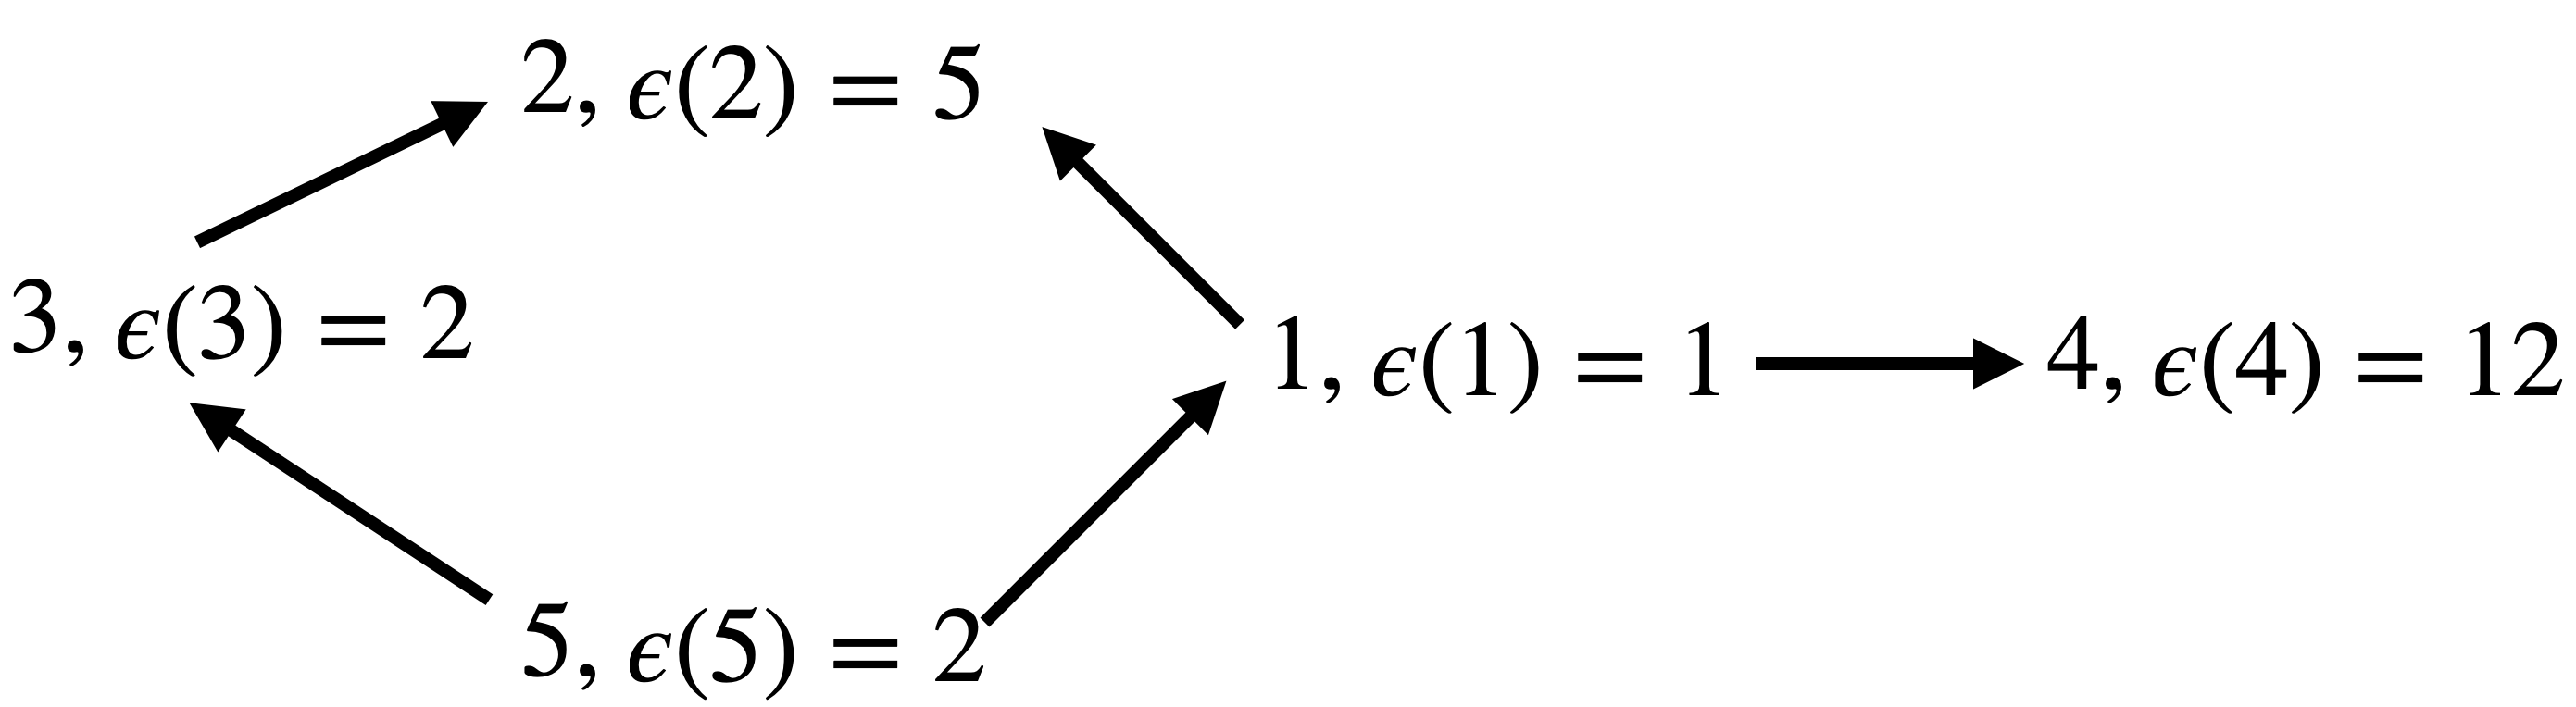
\includegraphics[scale=0.16]{Poset.png}
 \label{fig : poset}
 \end{center}
 %
 For any set $\mathcal{Z}\subseteq \PP^{\pm}$, we define the generating function \defn{$\Gamma_\mathcal{Z}([n], <_P, \epsilon)$} of the labelled weighted poset $([n], <_P, \epsilon)$ by
\begin{equation}
\label{eq : weightGamma}
\Gamma_\mathcal{Z}([n], <_P, \epsilon) = \sum_{f \in \calA_\mathcal{Z}([n], <_P)}\ \ \prod_{1\leq i \leq n}x_{|f(i)|}^{\epsilon(i)} .
\end{equation} 
 \end{definition}

\begin{proposition}{Decomposition of $\Gamma_\mathcal{Z}([n], <_P, \epsilon)$ into linear extensions}{prop.Gamma.linexts}
Let $P = ([n], <_P, \epsilon)$ be a labelled weighted poset.
Let $\calL\tup{P}$ be the set of all linear extensions of the poset $([n], <_P)$. Then,
\[
\Gamma_\mathcal{Z}([n], <_P, \epsilon)
= \sum_{([n], <_L) \in \calL\tup{P}} \Gamma_\mathcal{Z}([n], <_L, \epsilon) .
\]
\end{proposition}
 
 %%%%%%%%%%%%%%%%%%%%%%%%%%%%%%%%%%
\subsection{Universal quasisymmetric functions}
%%%%%%%%%%%%%%%%%%%%%%%%%%%%%%%%%%
\begin{definition}{Universal quasisymmetric functions}{def.universal}
Let $\alpha = (\alpha_1, \alpha_2, \ldots, \alpha_n)$ be a composition.
Let $\pi=\pi_1\dots\pi_n$ (in one-line notation) be a permutation in $S_n$.

Let $\defnm{P_{\pi,\alpha}} = ([n],<_\pi,\alpha)$ denote the labelled weighted poset composed of the labelled poset $([n], <_\pi)$ and the weight function
\[
\alpha : \pi_i \mapsto \alpha_i .
\]
\begin{center}
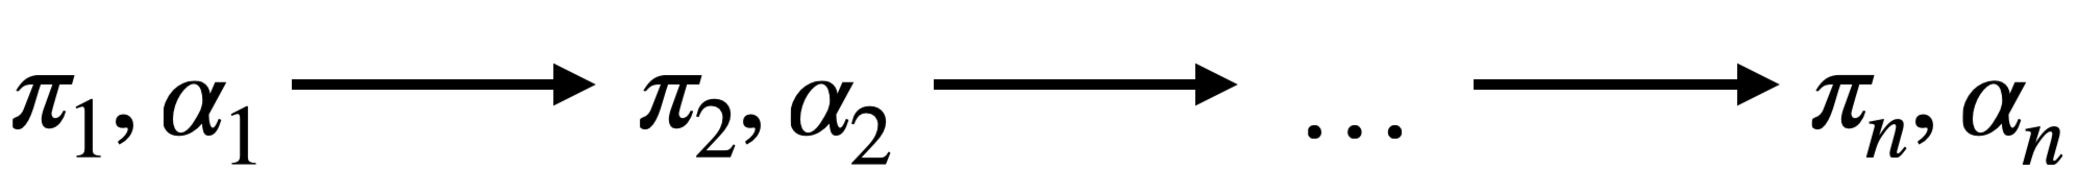
\includegraphics[scale=0.20]{PosetMonomial.pdf}
 \label{fig : monomial}
 \end{center}
We define the \defn{universal quasisymmetric function} $U^\mathcal{Z}_{\pi,\alpha}$ as the generating function
\begin{equation}
U^\mathcal{Z}_{\pi,\alpha} = \Gamma_\mathcal{Z}([n],<_\pi, \alpha).
\end{equation}
\end{definition}

So the $U^\mathcal{Z}_{\pi,\alpha}$s are the $\Gamma_\mathcal{Z}([n], <_P, \epsilon)$s for totally ordered $P$'s.
Thus, by Proposition~\ref{prop.Gamma.linexts}, each $\Gamma_\mathcal{Z}([n], <_P, \epsilon)$ is a sum of $U^\mathcal{Z}_{\pi,\alpha}$s.

The $U^\mathcal{Z}_{\pi,\alpha}$s include, as particular cases, all four bases we have seen so far (thus the ``universal''):

\begin{proposition}{Specialisation of universal quasisymmetric functions}{prop.spec}
\indent Let $n \in \NN$. Let \defn{$id_{n}$} and \defn{$\overline{id_{n}}$} denote the two permutations in $S_n$ given by $id_{n} = 1~2~3\dots n$ and $\overline{id_{n}} = n~n-1~n-2\dots 1$ (in one-line notation). Let \defn{$(1^n)$} be the composition $\tup{1, 1, \ldots, 1}$ of $n$. Then:
\begin{itemize}
\item For any $\pi \in S_n$, we have
\begin{align*}
U^\mathcal{\PP}_{\pi,(1^n)} = L_\pi, ~~~~~~U^\mathcal{\PP^\pm}_{\pi,(1^n)} = K_\pi .
\end{align*}
\item For any composition $\alpha$ with $n$ entries, we have
\begin{align}
U^{\mathcal{\PP}}_{\overline{id_{n}},\alpha} = M_{\alpha},
~~~~~U^{\mathcal{\PP^\pm}}_{id_{n},\alpha} = \eta_{\alpha}
\label{eq : UE}
\end{align}
(where we identify $\alpha$ with the appropriate weight function as in the definition above).
\end{itemize}

\end{proposition}

 %%%%%%%%%%%%%%%%%%%%%%%%%%%%%%%%%%
\subsection{Product rule}
%%%%%%%%%%%%%%%%%%%%%%%%%%%%%%%%%%
\begin{theorem}{Product of universal quasisymmetric functions}{thm.prod.universal}
Let $\mathcal{Z}$ be a subset of $\PP^{\pm}$.
Let $\pi$ and $\sigma$ be two permutations in $S_n$ and $S_m$, and let $\alpha = (\al_1,\dots,\al_n)$ and $\beta = (\be_1,\dots,\be_m)$ be two compositions with $n$ and $m$ entries.
The product of two universal quasisymmetric functions is given by
\begin{equation}
\label{eq : UU}
U^\mathcal{Z}_{\pi,\alpha}U^\mathcal{Z}_{\sigma,\beta}=\sum_{(\tau,\gamma)\in(\pi,\alpha)\shuffle(\sigma,\beta)}U^\mathcal{Z}_{\tau,\gamma} ,
\end{equation}
where the sum is over all ways to shuffle $\pi$ with $m + \sigma$ and -- using the same shuffle -- shuffle $\alpha$ with $\beta$.
\end{theorem}
% \begin{proof}
% The proof is iterative and uses the following decomposition of posets.
% %
% \begin{figure}[htbp]
% \begin{center}
 % 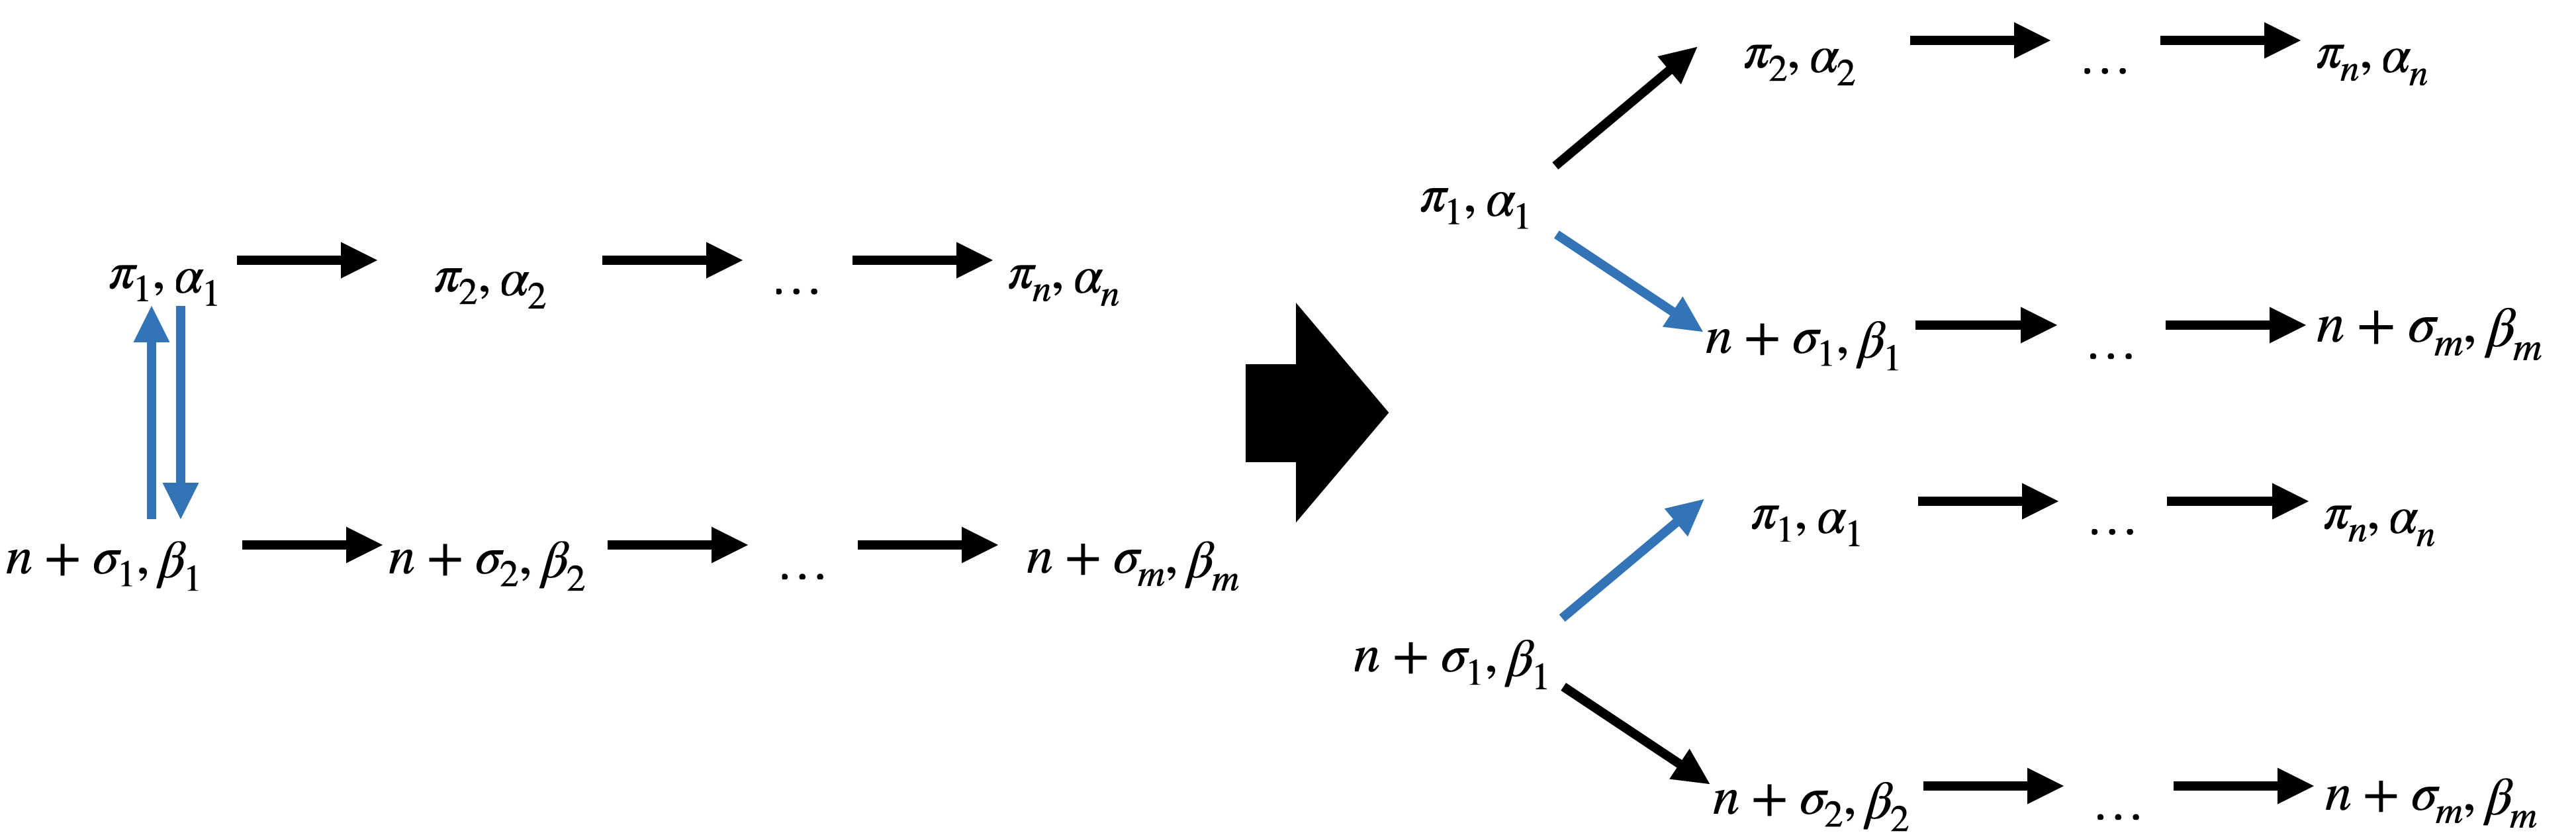
\includegraphics[scale=0.22]{PosetBij.png}\caption{Decomposition of a double chain weighted poset into two posets with one incomparable pair less.}
 % \label{fig : prodmonomial}
 % \end{center}
 % \end{figure}
 % %
% \end{proof}

%%%%%%%%%%%%%%%%%%%%%%%%%%%%%%%%%%
\subsection{Product of  enriched monomials}
%%%%%%%%%%%%%%%%%%%%%%%%%%%%%%%%%%
Let $\alpha$ and $\beta$ be two compositions with $n$ and $m$ entries. Equations (\ref{eq : UE}) and (\ref{eq : UU}) imply:
\begin{align}
\label{eq : MME}
\eta_\al \eta_\beta = U^{\PP^\pm}_{id_{n},\alpha}U^{\PP^\pm}_{id_{m},\beta}=\sum_{(\tau,\gamma)\in(id_{n},\alpha)\shuffle(id_{m},\beta)}U^{\mathcal{\PP^\pm}}_{\tau,\gamma} .
\end{align}
\begin{definition}{Composition reduction}{def.comp.reduc}
Let $\al = (\al_1, \dots, \al_n)$ be a composition with $n$ entries. Let $\al^{\downarrow\downarrow i}$ denote the following composition with $n-2$ entries:
\begin{equation*}
\al^{\downarrow\downarrow i} = (\al_1, \dots, \al_{i-2},{\al_{i-1}+\al_i+\al_{i+1}},\al_{i+2},\dots ,\al_n) .
\end{equation*}  
Furthermore, for any peak-lacunar subset $I\subseteq [n-1]$, we set $\al^{\downarrow\downarrow I}= \al$ if $I=\varnothing$ and
\[
\al^{\downarrow\downarrow I}
= \left( \left( \cdots \left( \al^{\downarrow i_k} \right) \cdots \right)^{\downarrow i_2} \right)^{\downarrow i_1} ,
\]
where $i_1, i_2, \ldots, i_k$ are the elements of $I \neq \varnothing$ in increasing order.
As an example, let $\al = (2,1,4,3,2)$. We have $\al^{\downarrow\downarrow 3} = (2,8,2)$ and $\al^{\downarrow \downarrow\{2,4\}} = (12).$

\end{definition}
%
\begin{theorem}{Universal quasisymmetric functions to enriched monomials}{thm.univ.enriched}
Let $\alpha$ be a composition with $n$ entries and $\pi$ a permutation in $S_n$. We have
\begin{equation}
\label{eq : U as sum}
U^{\PP^\pm}_{\pi,\al} = \sum_{I \subseteq \Peak(\pi)}(-1)^{|I|}\eta_{\al^{\downarrow\downarrow I}} .
\end{equation}
\end{theorem}
\begin{proof}[Proof (sketch).]
From the definition of  $U^{\PP^\pm}_{\pi,\al}$, one can obtain without too much trouble that
\begin{equation*}
U^{\PP^\pm}_{\pi,\al} = \sum_{\substack{i_1\leq i_2\leq\dots \leq i_n;\\j\in \Peak(\pi) \implies \lnot \left( i_{j-1}=i_{j}=i_{j+1}\right)}}2^{|\{i_1,i_2,\dots,i_n\}|}x_{i_1}^{\al_1}x_{i_2}^{\al_2}\dots x_{i_n}^{\al_n} .
\end{equation*}
By the inclusion-exclusion principle, this can be rewritten as
\begin{equation*}
U^{\PP^\pm}_{\pi,\al} =\sum_{I \subseteq \Peak(\pi)}(-1)^{|I|} \underbrace{\sum_{\substack{i_1\leq i_2\leq\dots \leq i_n;\\j\in I \implies  i_{j-1}=i_{j}=i_{j+1}}}2^{|\{i_1,i_2,\dots,i_n\}|}x_{i_1}^{\al_1}x_{i_2}^{\al_2}\dots x_{i_n}^{\al_n}}_{\substack{= \eta_{\al^{\downarrow\downarrow I}}\\}} .
\qedhere
\end{equation*}
\end{proof}
%
\begin{theorem}{Product rule for enriched monomials}{theorem : EEE}
Let $\al=(\al_1,\dots,\al_n)$ and $\beta=(\be_1,\dots,\be_m)$ be two compositions. Given a composition $\gamma$ obtained by shuffling $\al$ and $\be$ (we shall denote this by $\gamma \in \al\shuffle\be$), let $S_\beta(\gamma)$ be the set of the positions of the entries of $\beta$ in $\gamma$. Denote further $S_\beta(\gamma)-1 =\{i-1|i \in S_\beta(\gamma)\}$. Then,
\begin{equation}
\label{eq : EEE}
\eta_\al \eta_\beta
= \sum_{\substack{\gamma \in \al \shuffle \be ;\\
                   I\subseteq \left(S_{\be}(\gamma)\setminus (S_{\be}(\gamma)-1)\right) \setminus \left\{1\right\}}}
(-1)^{|I|}\eta_{\gamma^{\downarrow\downarrow I}} .
\end{equation}
The sum ranges not over compositions $\gamma$ but over ways to shuffle $\al$ with $\be$. Thus, the same $\gamma$ can appear in several addends of the sum.\\
As an example, one has
\begin{align*}
\eta_{(1,1)}\eta_{(2,3)} &= \eta_{(1, 1, 2, 3)} + \eta_{(1, 2, 1, 3)} -\eta_{(4, 3)} + \eta_{(2,1,1,3)}+\eta_{(1,2,3,1)}\\
&\qquad -\eta_{(1,6)}+\eta_{(2,1,3,1)}-\eta_{(2,5)}+\eta_{(2,3,1,1)}-\eta_{(6,1)},\\
\eta_{(1,2)}\eta_{(2)} &=  \eta_{(2,1,2)} +   2\eta_{(1,2,2)} - \eta_{(5)}.
\end{align*}
\end{theorem}
\begin{proof}[Proof (sketched).]
Recall \eqref{eq : MME}, and rewrite the right-hand side using \eqref{eq : U as sum}.
Let $(\tau,\gamma)$ be a coshuffle in $(id_n,\al)\shuffle(id_m,\be)$. The index $i$ belongs to $\Peak(\tau)$ if and only if $\tau_i$ is a letter of $n+id_m$ and $\tau_{i+1}$ is a letter of $id_n$ and we have $i > 1$. That is, if and only if $i$ is the index of an entry of $\beta$ in $\gamma$ and $i+1$ is the index of an entry of $\al$.
Thus, $\Peak(\tau) = \left(S_{\be}(\gamma)\setminus (S_{\be}(\gamma)-1)\right) \setminus \left\{1\right\}$.
Therefore, we obtain \eqref{eq : EEE}.
\end{proof}
\printbibliography
\end{document}